\documentclass{beamer}

\usepackage{graphicx}
\usepackage{listings}

\title{MongoDB Basics}
\author{Michael Albertson}
\date{2015-05-12}

\begin{document}


\begin{frame}

\maketitle

\end{frame}


\begin{frame}{What is No-SQL?}

\begin{itemize}
\item Denormalized
\item Distributed with high scalability
\item BASE instead of ACID % http://www.eecs.berkeley.edu/~brewer/cs262b-2004/PODC-keynote.pdf
\item CAP Theorem
\item Not just SQL
\end{itemize}

\end{frame}


\begin{frame}{What is MongoDB?}

\begin{itemize}
\item Named for Humongous
\item High scalability
\item Fast writes
\item BSON
\item Geospatial indexing
\item Aggregation (map and reduce)
\end{itemize}

\end{frame}


% I'm a bit less certain about this frame.
\begin{frame}{My background with MongoDB}

\begin{itemize}
\item XY Maps search engine
\item DUI cam server
\end{itemize}

\begin{center}

\includegraphics[scale=.5]{xy-logo.png}
\end{center}

\end{frame}


\begin{frame}{Why you should use it}

\begin{itemize}
\item Ease of use
\item JavaScript on the backend
\item Systems that may not need ACID
\end{itemize}

\end{frame}


\begin{frame}{The reasons not to use it}

\begin{itemize}
\item Aggregation is slow
\item XSS on the backend
\item There are still databases that should be relational
\end{itemize}

\end{frame}


\begin{frame}

\begin{center}
   Installation Demo
\end{center}

\end{frame}


\begin{frame}

\begin{center}
   Shell Demo
\end{center}

\end{frame}


\begin{frame}{Geospatial Indexing}

\begin{itemize}
\item Spherical or planar coordinates
\item All spherical coordinates must be WGS 84
\item Uses geohashing
\item Only allows 2 dimensions
\item 2dsphere requires GeoJSON
\end{itemize}

\end{frame}


\begin{frame}

\begin{center}
   Demo
\end{center}

\end{frame}


\begin{frame}{Suggested reading}

\begin{itemize}
\item MongoDB: the Definitive Guide
\item No ever got fired for using Hadoop in a cluster \url{http://research.microsoft.com/jump/163083}
\item Towards robust distributed systems \url{https://www.cs.berkeley.edu/~brewer/cs262b-2004/PODC-keynote.pdf}
\end{itemize}

\begin{center}
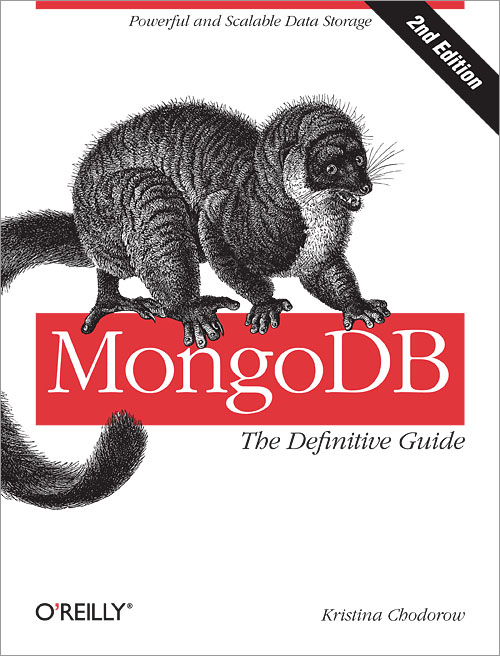
\includegraphics[scale=0.75]{mongo-cover.jpg}
\end{center}

\end{frame}


\begin{frame} % Conclusion

\begin{center}
   Any questions?
\end{center}

This talk should be available on GitHub.

If you want to contact me:
\begin{itemize}
\item Email: mdalbertsonjr@gmail.com
\item Twitter: @mdalbertsonjr
\item Radio: KJ6RAS
\end{itemize}

\end{frame}

\end{document}
